\documentclass{ctexart}
\title{注意力模型综述}
\author{姚兴虎}
\date{\today}

\usepackage{geometry}
\geometry{a4paper,scale=0.8}
\usepackage{amsfonts}
\usepackage{amsmath}
\usepackage{amssymb}
\usepackage{subfig}
\usepackage{dsfont}
\usepackage{graphicx, dblfloatfix}
\newtheorem{Def}{\hspace{2em}定义}
\newtheorem{Theo}{\hspace{2em}定理}
\begin{document}
\maketitle
\section{简介}
自从被提出用以解决机器翻译问题以来,注意力模型(Attention Model,AM)现在已经成为神经网络研究中的一个非常重要的研究领域。注意力模型已经被广泛的应用到自然语言处理,统计学习语音识别和计算机视觉等人工智能相关领域。

注意力机制的灵感来源可以归结到人对环境的生理感知上来。比方说,我们的视觉系统更倾向于去挑选影像中的部分信息进行集中分析而忽略掉图像中的无关信息。与此类似,很多设计到语言,语音和视觉的问题中都包含与研究任务密切相关的信息,同时也包含着一些无关的信息。比方说,在文本翻译和总结任务中,可能只有输入序列的某些单词与我们的下一个预测输出值有关;在图像标注任务中,可能某些局部信息与下一个标注单词联系更为密切。注意力机制将这种相关系进行了整合,允许模型动态地去关注输入的特定部分从而更为有效地完成手头的任务。下图表示了引入注意力模型进行情感分类的一个例子,从中可以看出第一句和第三句与我们的任务更为相关。更具体来说,单词\textit{delicious}和\textit{amazing}与情感分类问题更为相关。
\begin{figure}[htb!]
	\centering
	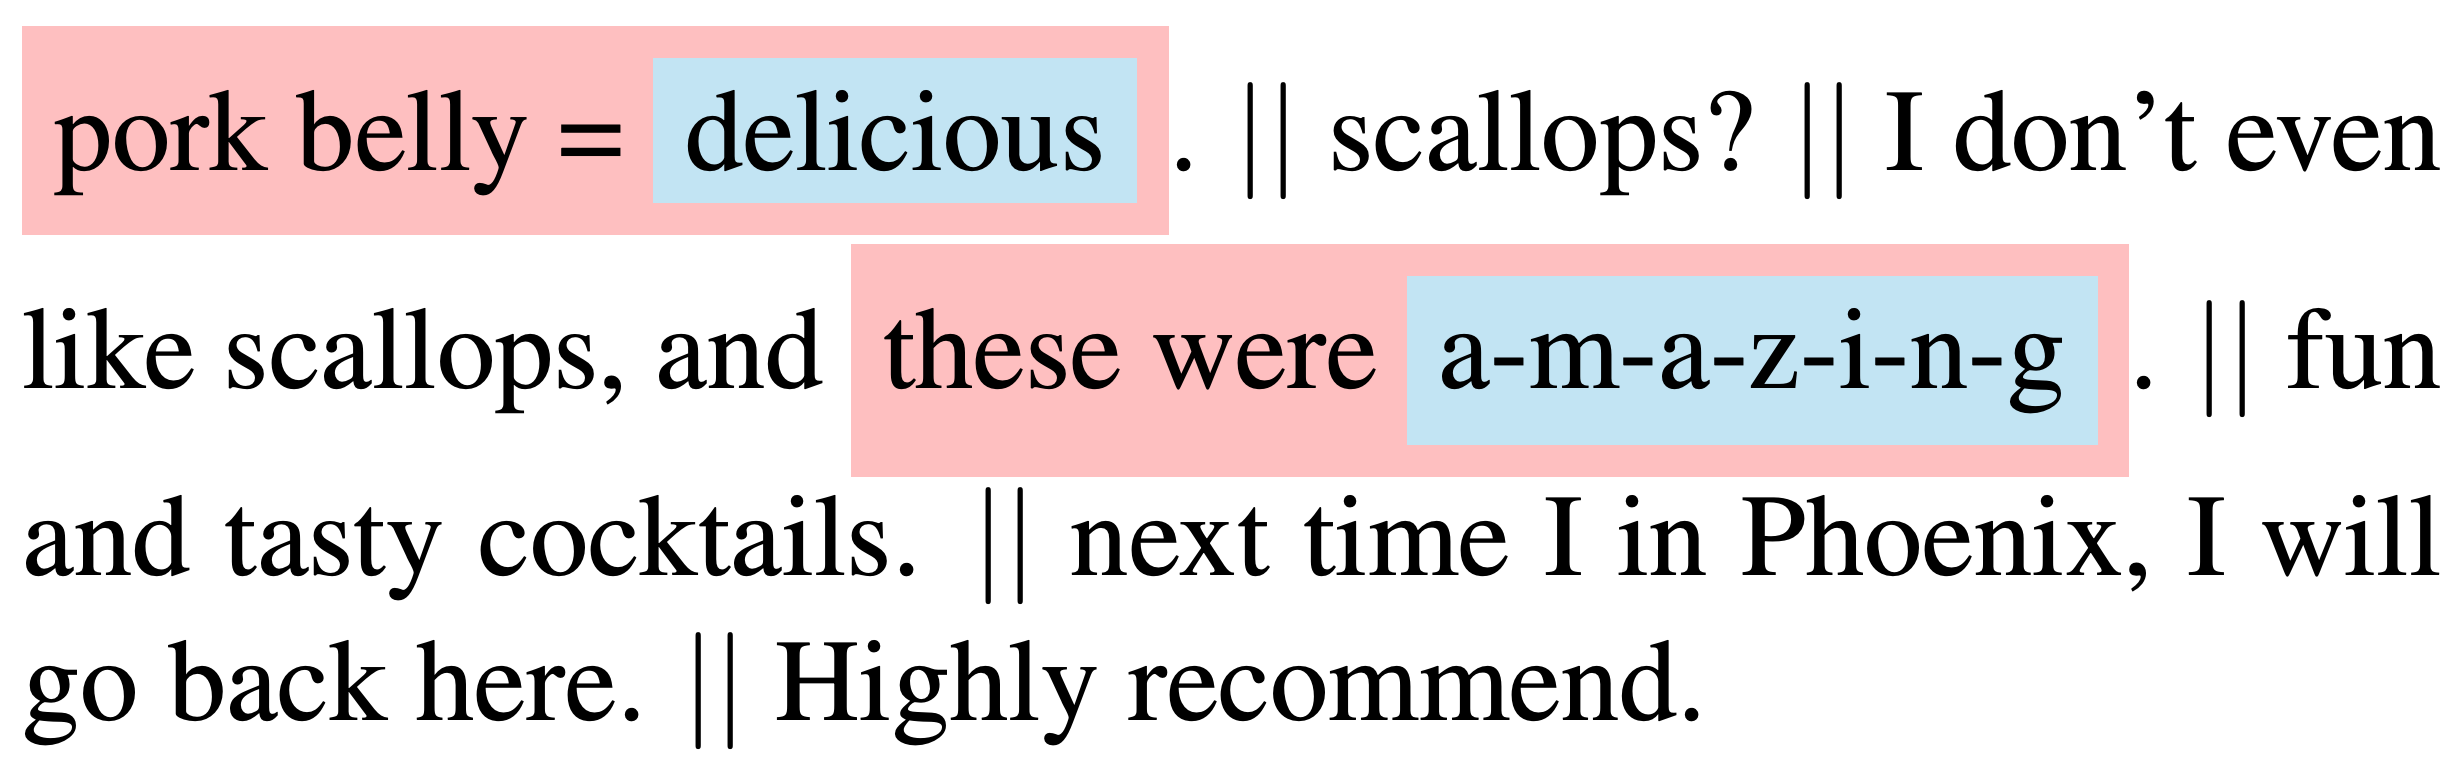
\includegraphics[scale=0.38]{document.png}
	\caption{加入注意力机制用于情感分类的一个例子}
\end{figure}
在神经网络结构中加入注意力模型主要是基于三点考虑:首先是这些模型在众多的任务中取得了非常好的性能,比方说机器翻译、问答系统、情感分析、词性标注选民分析和问答系统。然后,在提升模型性能的同时,注意力机制增加了神经网络结构的可解释性。由于传统的神经网络是一个黑盒模型,因此提高其可解释性对机器学习模型的公平性、可靠性和透明性的提高至关重要。第三,其能够帮助缓解递归神经网络中的一些缺陷,比方说随着输入序列长度的增加导致的性能下降和对输入的顺序处理所导致的计算效率低下。本文的目的在于对注意力模型进行一个简单且易理解的介绍。
\section{注意力模型}
如图2(a)所示,一个经典的序列模型(sequence-to-sequence)包含一个编码部分和一个解码部分。编码器通常采用一个循环神经网络结构来对序列的输入$\left\{x_1,x_2,\cdots,x_T\right\}$进行编码得到一组固定长度的编码向量$\left\{h_1,h_2,\cdots,h_T\right\}$。解码器同样利用一个RNN结构读取单个输入$h_T$然后一个接一个的进行输出得到一个输出序列$\left\{x_1,x_2,\cdots,x_{T'}\right\}$。其中$T$和$T'$分别代表输入和输出序列的长度。在每个位置$t$,$h_t$和$s_t$分别代表该位置编码器和解码器的隐藏状态。
\subsection{传统编码-解码结构的缺点}
这一编码-解码结构有两个主要的缺陷。首先便是编码器必须将所有的输入信息压缩成固定长度的向量$h_T$。使用这种简单的定长编码来表示更长和更复杂的输入往往会造成输入信息的丢失。其次,这样的结构不能对输入序列和输出序列的对应关系进行建模,而这种对应在机器翻译和文本摘要等任务中十分重要。直观上来说,在序列任务中,输出序列的每个位置可能会受到输入序列的特定位置的影响。然而,经典的解码结构在产生输出时并不会考虑这种对应关系。
\begin{figure}[htb!]
	\centering
	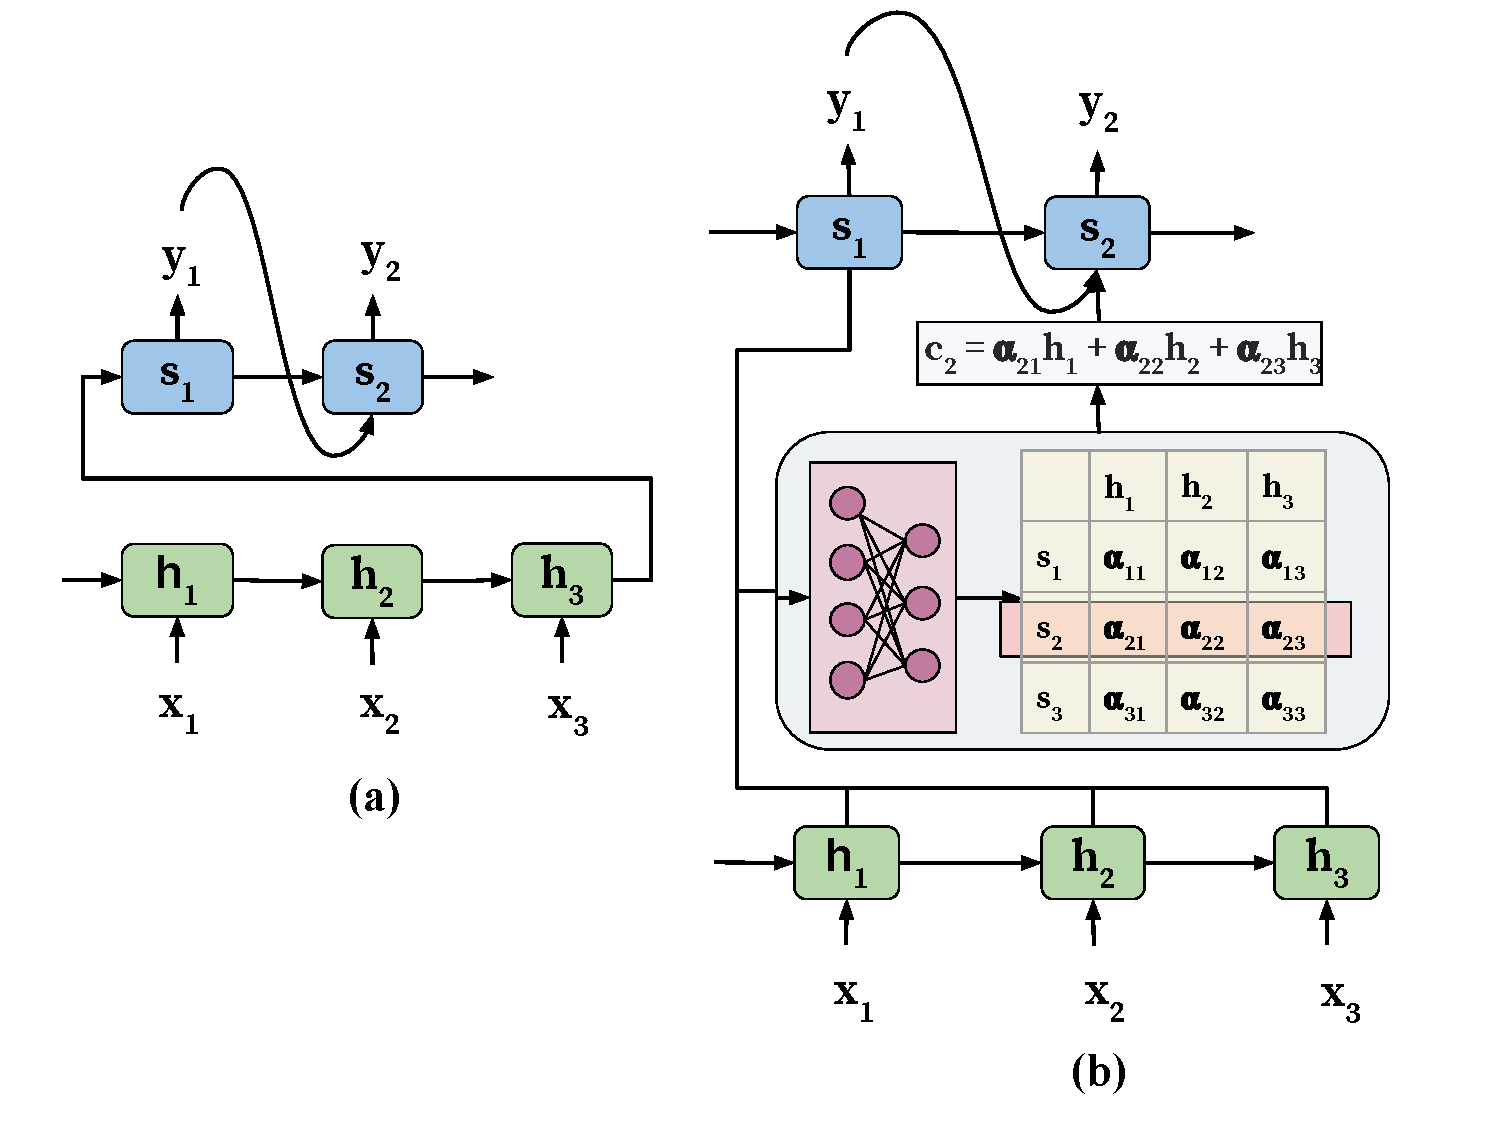
\includegraphics[scale=0.6]{sec2f.pdf}
	\caption{编码器-解码器结构:(a)传统结构 (b)加入注意力机制的模型的结构}
\end{figure}
\subsection{注意力模型的核心想法}
注意力模型通过允许解码器访问所有编码器产生的输出$\left\{h_1,h_2,\cdots,h_T\right\}$来克服传统结构的上述两大缺点。其核心思想是对编码器的所有输出进行加权组合后输入到当前位置的解码器中来影响解码器的输出。通过对编码器的输出进行加权,在实现输入与输出的对齐的同事还能够利用更多的原始数据的上下文信息。
\subsection{注意力机制的引入}
引入注意力机制的模型的结构如图2(b)所示。注意力模块能够自动地学习权重$\alpha_{ij}$用来捕捉编码器隐藏状态$h_i$和解码器隐藏状态$s_j$的相关性。习得的这些注意力权重将会被用来构建一个上下文向量$c$来作为解码器的输入。在解码器的每个位置$j$,上下文向量$c_j$是由注意力权重对所有的编码器的隐藏状态进行加权求和进行得到的,即:$c_j=\sum_{i=1}^{T}\alpha_{ij}h_i$。于是,这一上下文向量其实为解码器提供了一种访问整个输入序列并且关注序列中的特定相关位置的一种机制,我们称这种机制为注意力机制。
\subsection{注意力权重的学习}
注意力权重的学习是通过在原始的网络结构中增加一个前馈网络来实现的。这一前馈网络的注意力权重的值$\alpha_{ij}$是编码器隐藏状态值$h_j$和解码器内部隐藏状态值$s_{i-1}$的函数。该前馈网络可以与之前的网络结构一起进行训练。
该权重值可以通过下面的表达式算出:
\begin{align*}
e_{ij} &= v_a^Ttanh(W_as_{i-1}+U_ah_j)\\
\alpha_{ij} &= \frac{exp(e_{ij})}{\sum_{k=1}{T_x}exp(e_{ik})} 
\end{align*}
其中$v_a,W_a,U_a$是注意力网络的权重值。
\section{注意力模型的分类}
\subsection{序列的数量}
目前为止我们考虑的注意力模型是由单个输入序列和与之相对应的单个输出序列组成的,我们将这种注意力模型成为\textit{\textbf{单注意力模型}}。这种注意力机制常被用在候选状态(如上文中编码器的输出h)和查询状态(解码器的隐藏状态s)属于两个不同的输入输出序列的任务中。机器翻译、文本摘要,图像捕捉和语音识别任务中的大部分基于注意力机制的模型采取了这一单注意力模型结构。


\textit{\textbf{协注意力模型}}则能够处理多个输入序列并协同学习这些不同输入序列之间的注意力权重来捕捉不同输入之间的内在关系。比方说在图像问答任务中,除了我们对输入图像进行注意力建模之外,我们还能够对问题的文本进行注意力建模。这是因为在问题的文本序列中,每个单词的对如何回答该问题所起的权重不一样。进一步说来,对图像和问题文本都进行基于注意力机制的建模能够起到一个协同互补的作用,这能够帮助我们同时捕捉到图像中的关键区域和问题中的关键词。


此外,对于文本分类和推荐任务,其输入是一个序列而输出不是一个序列。在这种场景下,注意力机制可以用来捕捉输入序列中的每个单元(比如每个单词)和该输入序列中的其他单元之间的联系。在这种情形下,注意力模型的候选状态和查询状态为同一个序列,我们将基于这种机制的注意力模型称为\textit{\textbf{自注意力模型}}。
\subsection{抽象的层数}
在最一般的情形下,注意力权重是仅仅是由注意力模型的原始的输入序列算出来的,这一注意力模型可被称为\textit{\textbf{单层注意力模型}}。另一方面,我们可对输入序列进行多次抽象,这样可以使得底层抽象的上下文向量成为下一次抽象的查询状态。这种对输入数据叠加若干层注意力模块实现对序列数据多层抽象的方法可被称为\textit{\textbf{多层注意力模型}}。更具体地来说,多层注意力模型又可按照模型的权重是自顶向下学习还是自底向上学习的方式进行划分。


多层注意力机制的一个典型应用是通过对文本进行两层抽象实现对文本的分类。这一模型称为“层次和注意力模型(Hierarchical Attention Model,HAM)”。文本是由不同的句子组合而成的,而每个句子又包含不同的单词,HAM能够对文章这种自然的层次化结构进行抽取。具体来说,其首先对每个句子建立一个注意力模型,该注意力模型的输入是每个句子中的基本单词,从而得到这个句子的特征表示;然后将句子的特征的表示输入到后续的注意力模型中来构建整段文本的特征表示。这一最后得到的整段文本的特征表示可以用于后面分类任务分类器的输入。


上一小节提到的协注意力机制也可以看做一种多层注意力模型。在下图所示的图像问答任务中,将基于图像的注意力模型和基于文本的注意力模型进行协同训练,而基于文本的注意力模型实际上完成了单个单词的抽象,短语的抽象以及整个问题的抽象这一层次化的过程。
\begin{figure}[htb!]
	\centering
	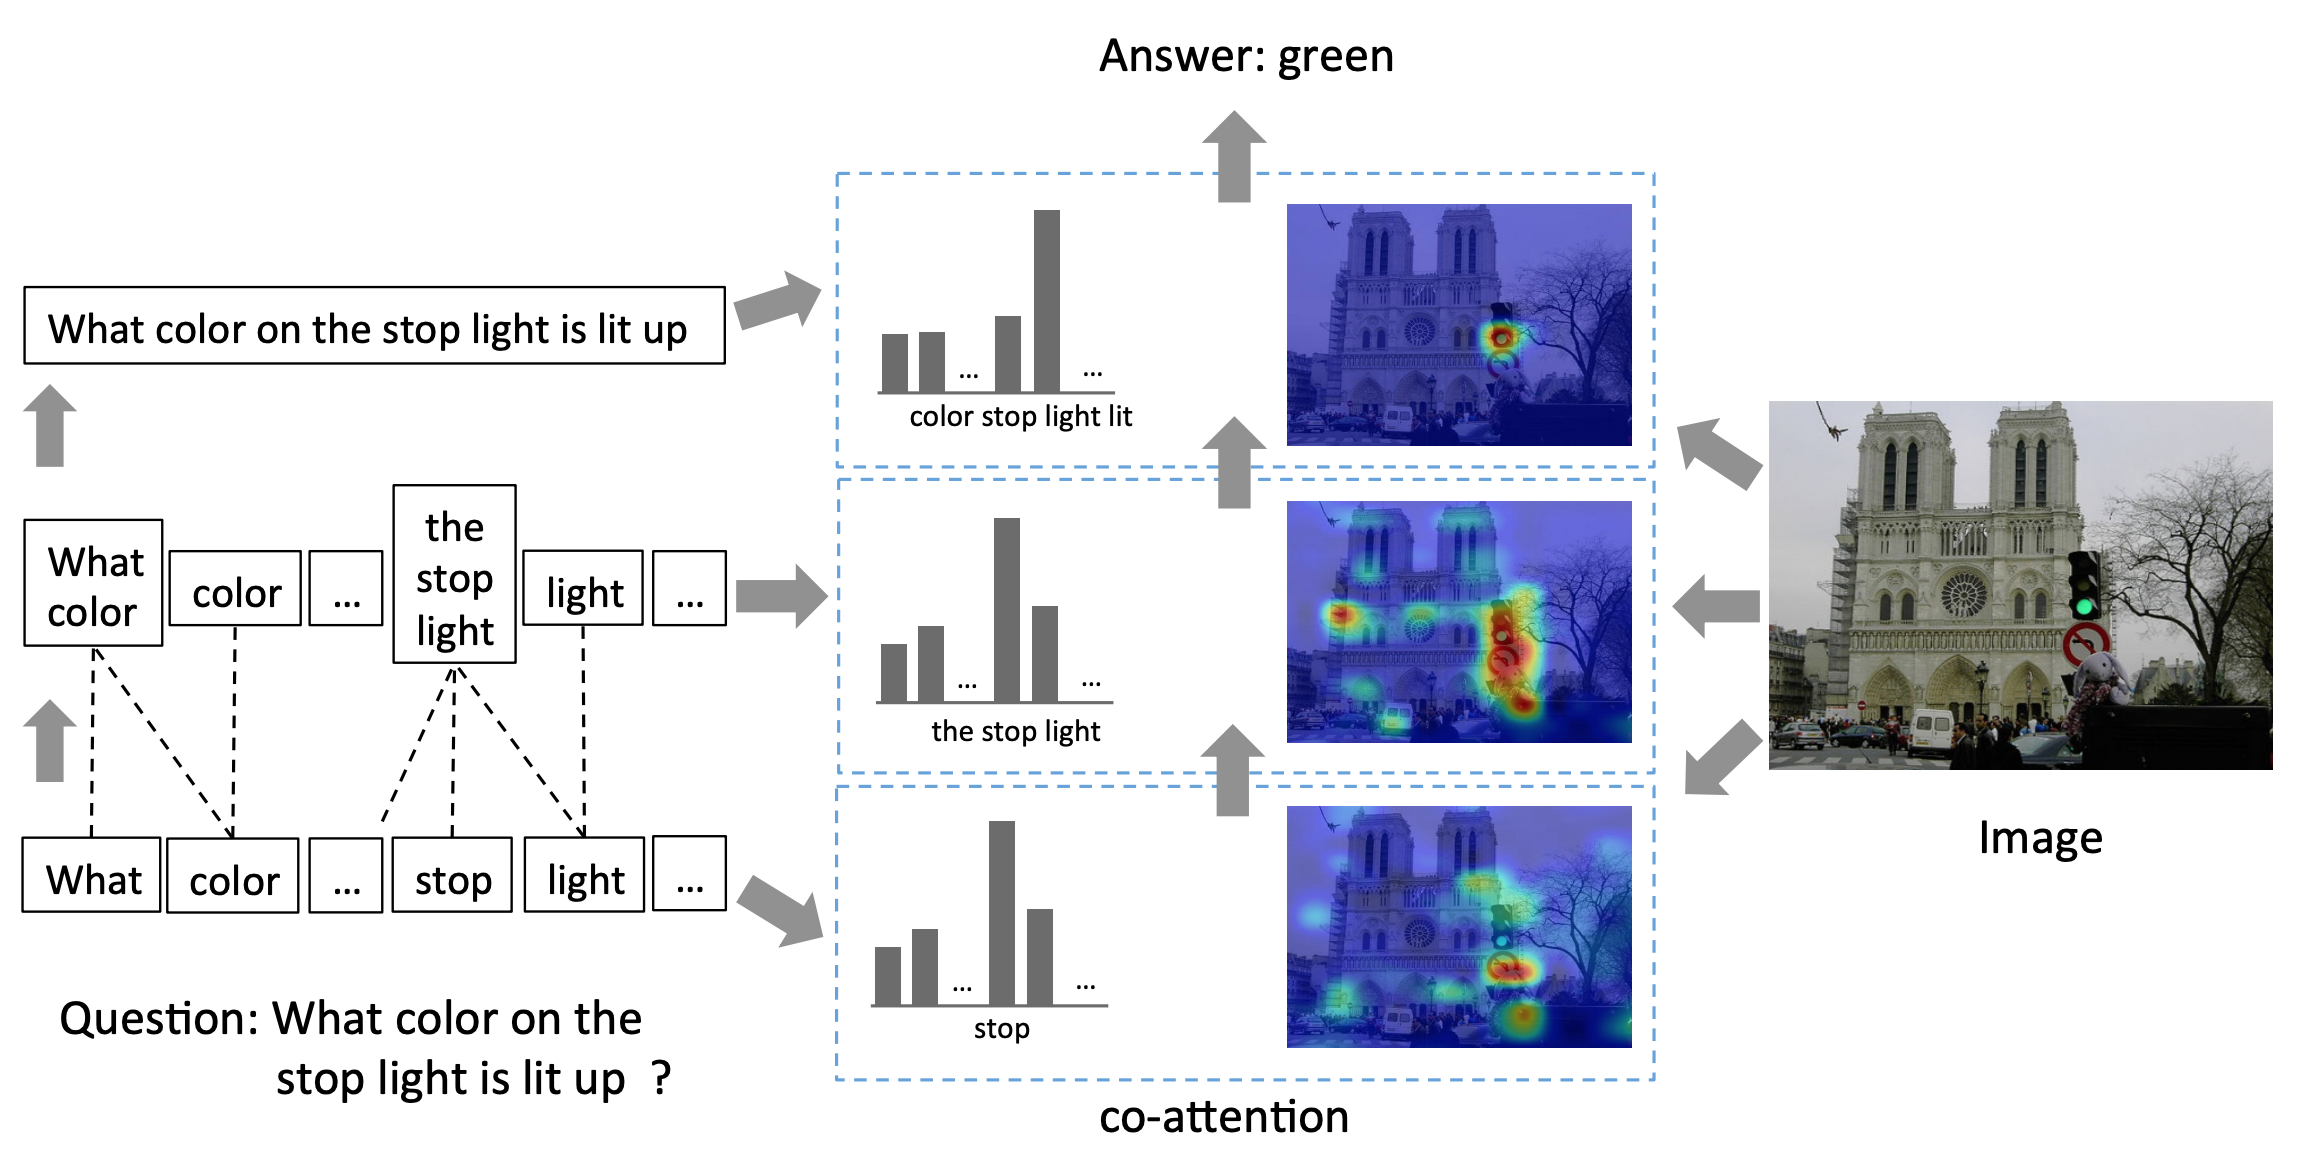
\includegraphics[scale=0.4]{co-multi.png}
	\caption{图像问答问题中的注意力模型的一种构建方法}
\end{figure}
\subsection{输入序列的单位数量}
在这种分类方法中,我们根据构建注意力模型时所用到的输入序列的位置和基本单位的长度来分类。最开始的文本翻译任务中,上下文向量是通过对输入序列的所有数据进行编码后的候选向量进行线性组合得到的,这种利用了全部输入信息的方法可被称为
\textit{\textbf{软注意力模型}}。这种软注意力模型能够有效地对神经网络进行反向传播的计算,但是也带来了平方级的计算代价。与之对应的是一组\textit{\textbf{硬注意力模型}},其上下文向量是通过随机候选的部分单元输入到注意力模型得到的,该方法降低了计算代价但同时对输入序列的随机选择使得整体框架变得不可微从而很难优化。这种硬注意力模型的缺陷可以借鉴变分学习方法以及强化学习中的策略梯度法进行克服。此外还有一种介于上述二者之间的注意力模型,一种称之为局部注意力模型的方法事先在输入序列中选择一个注意点,然后在这一点及其周围的数据点上构建一个局部的注意力模型。注意点的选择可以通过简单的对其方式也可以由学习算法得到。这一局部注意力机制实现了对计算代价和模型可微性的一种权衡。
\subsection{特征表示的数量}
在大多数的应用场景下,我们只会对输入数据进行一种特征表示。然而在有些场景下,对输入数据进行单一的特征表示可能不能够为后续的过程提供足够的信息。在这种情形下,我们可以对同样的输入数据进行多种特征表示。利用注意力机制可以为这些不同的特征表示指定相关的权重,从而丢弃掉输入数据中的噪声信息和重复冗余信息。我们称这种模型为\textbf{\textit{多表示注意力模型}}。这种多表示注意力模型能够决定不同特征表示的权重从而有助于后面对这一表示的应用。最后得到的输入的特征表示是多个特征表示的加权组合,这一模型的一个优势在于针对不同的后处理任务能够决定哪些特征表示更适合当前的任务场景。


基于类似的想法,还有一种称为\textbf{\textit{多维度注意力模型}}的方法。其核心观点是对特征表示向量的各个维度之间的依赖关系进行建模,这样我们便能够选择特征中更为有用的属性来帮助我们处理后续的任务。这一思想在自然语言处理领域至关重要因为相同的单词往往会出现多义性。
\section{加入注意力机制的神经网络结构}
在这一节我们介绍三种加入注意力机制的神经网络结构:(1)编码器-解码器结构;(2)针对单输入序列的记忆网络;(3)使用注意力机制来绕过循环神经网络中的顺序处理。
\subsection{编码器-解码器结构}
编码器-解码器结构常被用来处理机器翻译问题,自从2014年研究人员在这一结构中加入注意力网络从而大大提高了机器翻译性能以来,这一结构便成为非常流行包含注意力机制的网络结构。


一个有趣的事实是,注意力模块可以接受任何输入表示,并将其缩减为一个固定长度的上下文向量,以便在解码步骤中使用。因此,它允许将输入表示与输出解耦。人们可以利用这一优势引入混合编解码器,其中最流行的是卷积神经网络(CNN)作为编码器,而RNN或长短时记忆(LSTM)作为解码器。这种结构特别适用于许多多模态任务,如图像和视频字幕、视觉问题回答和语音识别。然而并不是所有输入和输出均为序列数据的问题都可以用这种编码器解码器结构解决。针对其他具体的任务场景还需设置不同的结构来将注意力模型与之结合在一起,对此类问题不再进行深入探讨。
\subsection{记忆网络}
问答和聊天机器人等任务场景要求程序能够从已有的一个知识数据库中进行学习。这时网络的输入是一个知识数据库和一个查询指令,其中知识库中的某些内容与我们的查询息息相关。端到端的记忆网络通过使用一组记忆模块来存储这一知识数据库,并且利用注意力机制来寻找这一知识数据库中与我们的查询更为密切的知识。在网络中加入这一注意力机制不会破坏网络的连续性因而不会增加优化的成本。这种端到端的记忆网络可以看做是对注意力模型的一种泛化,因为其不是对单个序列进行建模,而是对通过大量的序列对这些序列中的知识数据库进行建模。
\subsection{不含RNN的网络结构}
循环神经网络在编码的过程中以来与对数据的顺序处理,这使得其计算效率低并且不能顺序计算。为了克服这一问题,研究着提出了一种转换器(Transformer)结构,这一结构中编码器和解码器被压缩为由两个子层组成的相同结构:位置相关(Position-wise)的前馈网络和多头自注意层。


位置相关的前馈网络:由于输出的数据是带有顺序关系的,因此我们要求我们的模型能够捕捉到输入序列的顺序关系的同时不用计算代价较高的循环神经网络或者卷积网络。为了解决这一问题,我们可以设计一种前馈网络使之在编码阶段对输入的数据进行编码的同时对其位置信息进行编码。


多头自注意机制:在每个子层中使用自注意机制来关联输入数据及其在相同输入序列中的位置。此外,注意力被称为多头是因为几个注意力层是并行堆叠的,具有相同输入的不同线性变换。这有助于模型捕获输入的各个方面,并提高其表达能力。


转换器结构实现了并行处理、更短的训练时间和更高的转换精度,而没有任何重复组件。然而,位置编码只能很弱地包含位置信息,而且可能不适用于对位置变化更敏感的问题。不含RNN的结构还在不断被设计提出用来解决不同的问题。
\section{注意力机制的可解释性}
人们对人工智能模型的可解释性有着巨大的兴趣,这是由模型的性能、透明度和公平性驱动的。然而,神经网络,尤其是深度学习结构因其不可预测性而受到批评。从可解释性的角度来看,注意力模型特别有趣,因为它允许我们直接检查深度学习体系结构的内部工作。针对输入和输出均为一个序列的问题,注意力模型的一个重要假设是学习得到的注意力权重体现了当前需输出的数据与输入序列的某些特定位置数据的相关性。为了验证这一假设,我们可以通过对一组输入输出序列对进行可视化。


如图4(a)所示,研究人员将注意力权重可视化,尽管不同语言的主语-动名词位置不同,但法语和英语的句子自动对齐的效果很明显。在一般情况下,注意模型通过正确地将海洋环境与海洋环境进行比对,显示出非单调的一致性。图4(b)显示了注意力权重可以帮助重新记录用户的兴趣。用户1似乎更喜欢“卡通”视频,而用户2更喜欢“动物”视频。最后,研究人员提供了对图像字幕任务中生成的文本有显著影响的相关图像区域(即高注意权重)的大量可视化列表(如图4(c)所示)。
\begin{figure*}[!h]
	\centering
	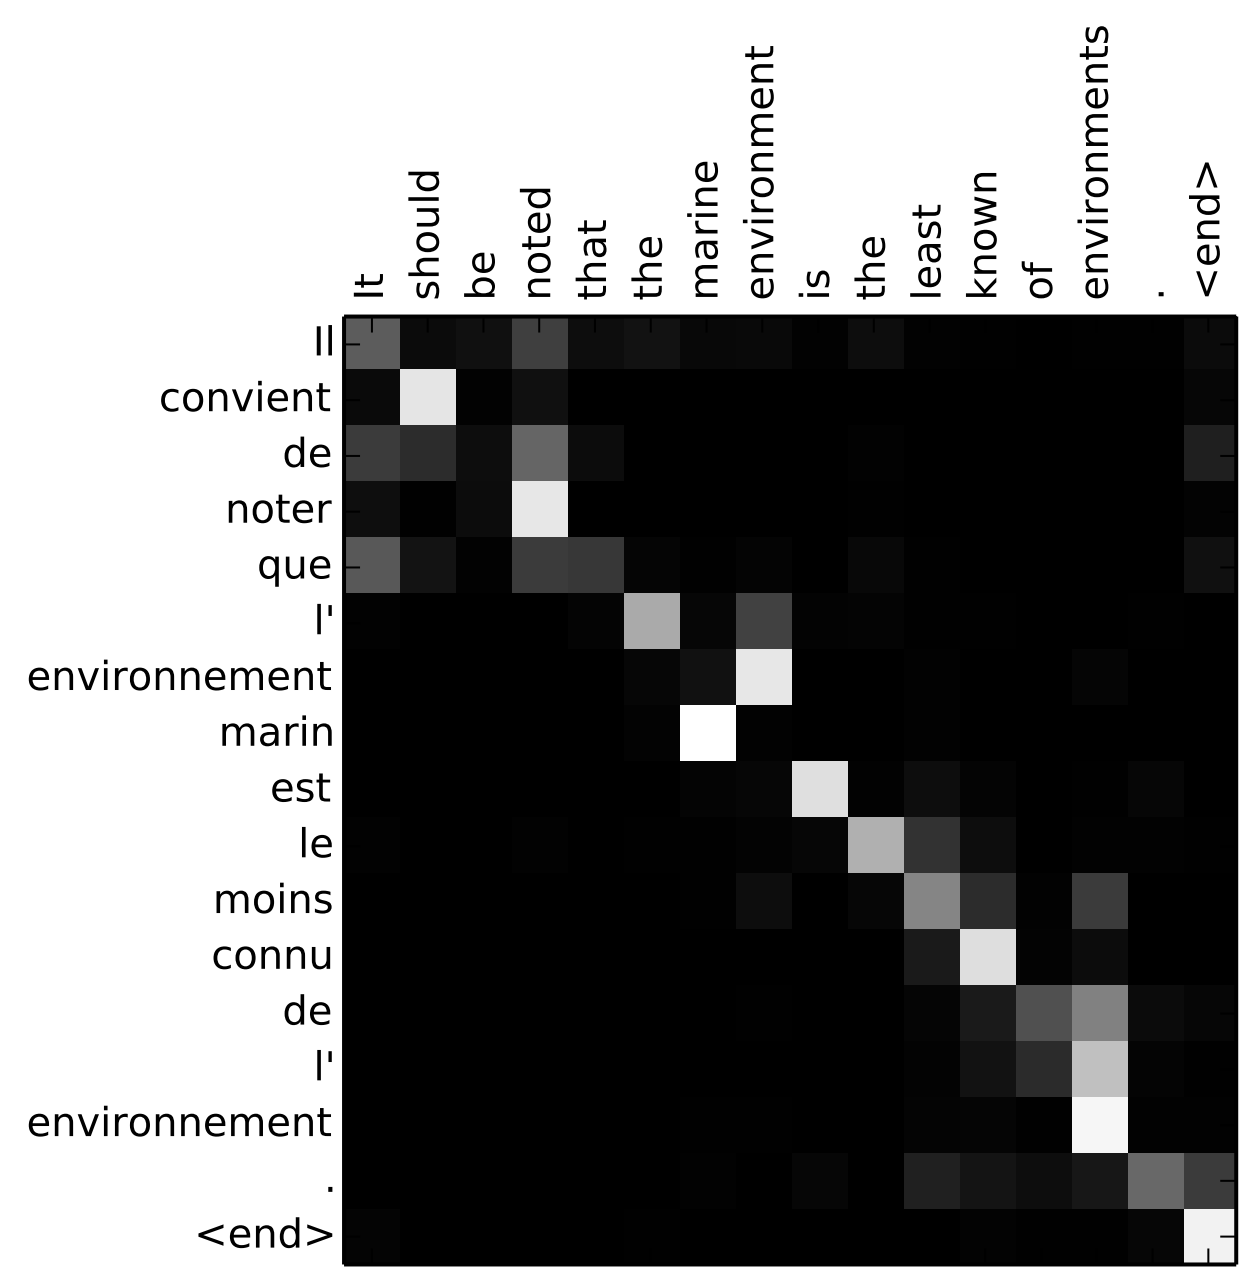
\includegraphics[width=4.5cm, height=4cm]{alignment.png} 
	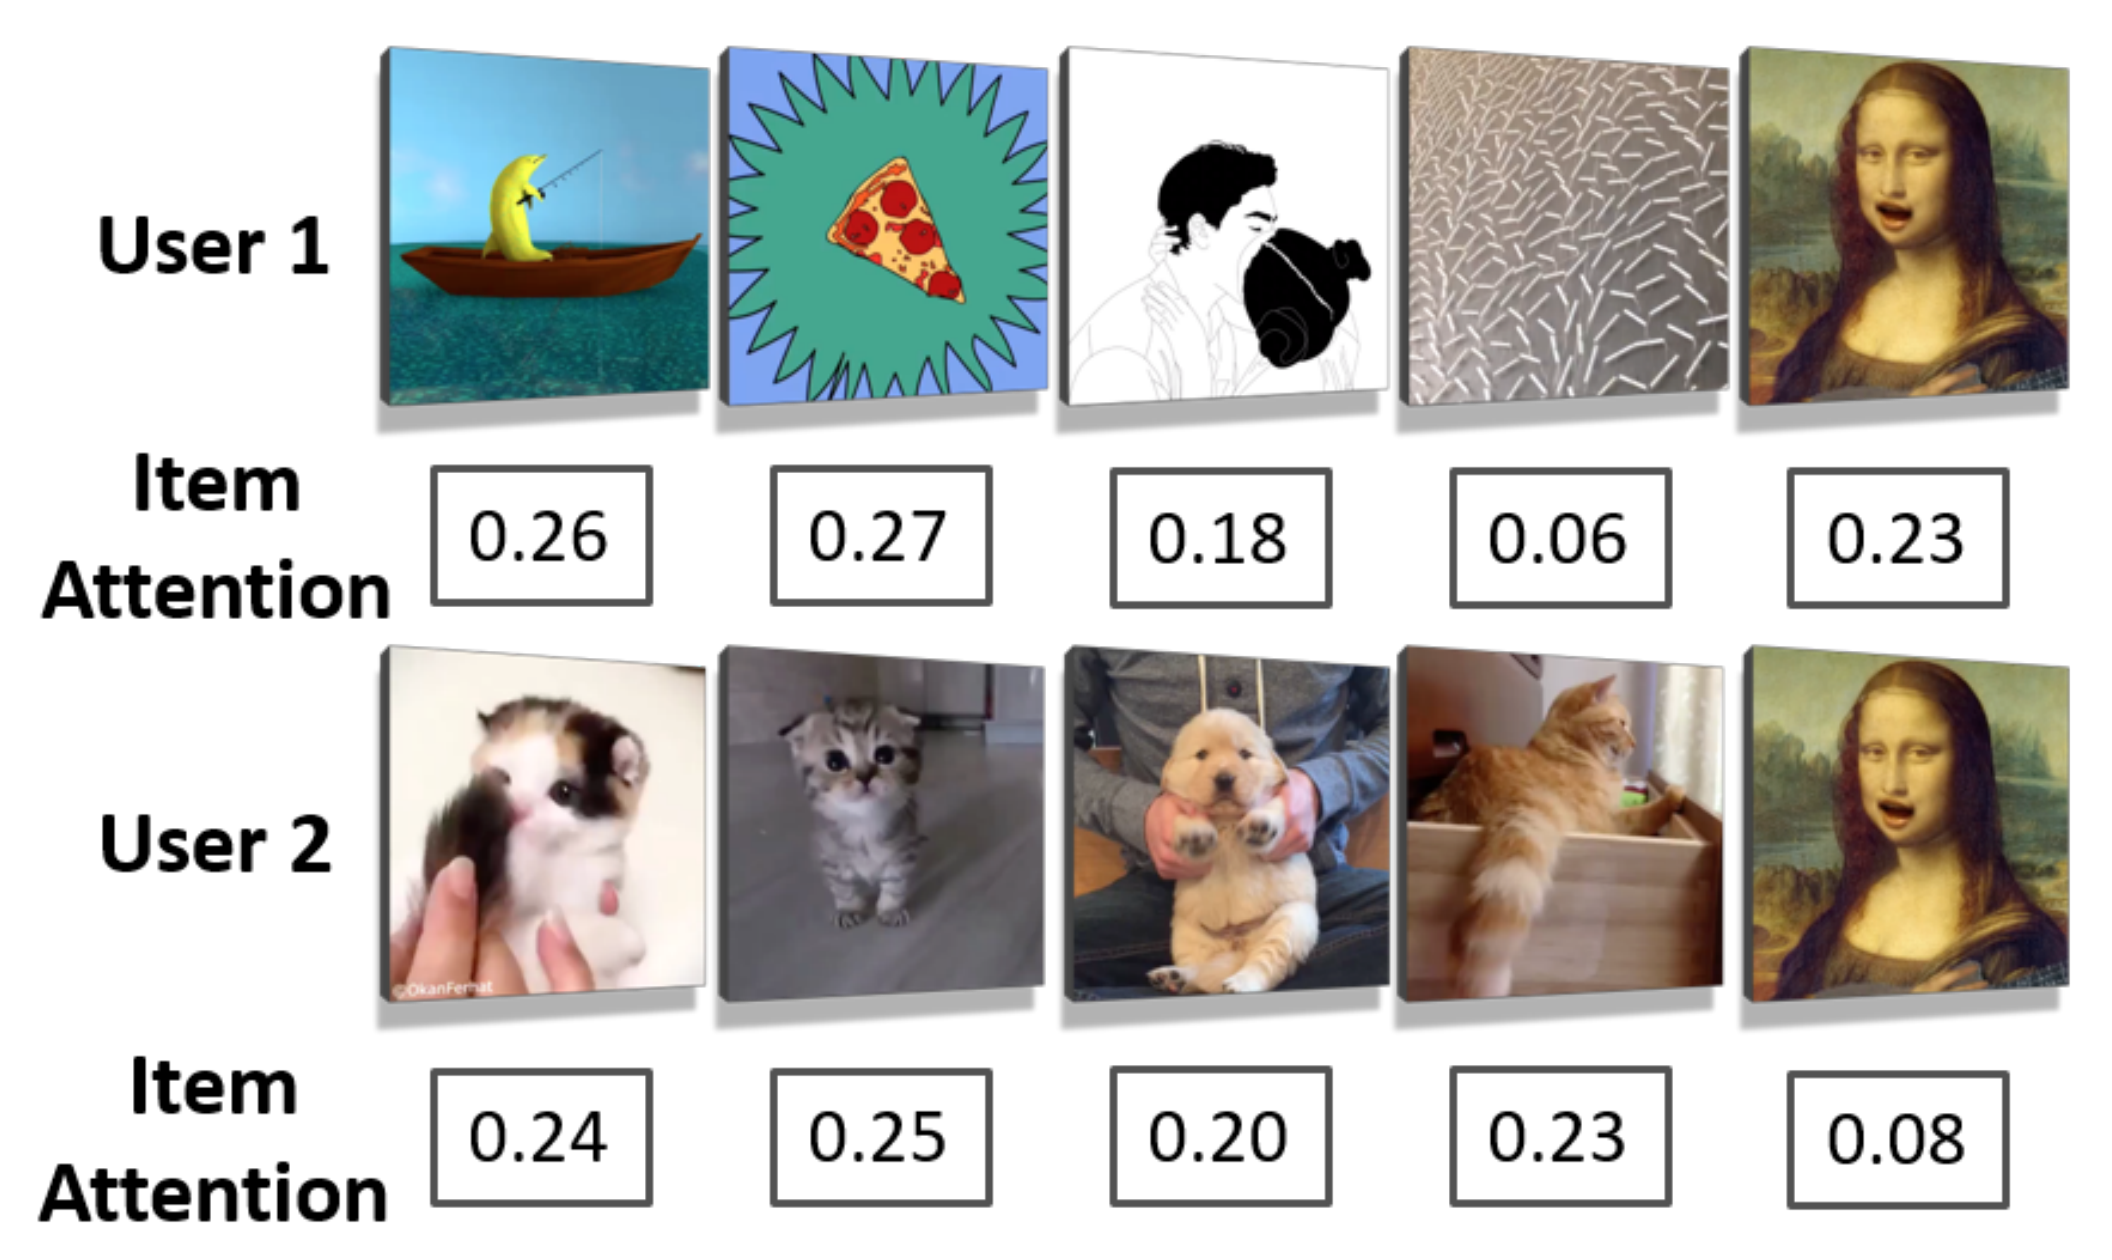
\includegraphics[width=5 cm, height=3.75cm]{rec.png}
	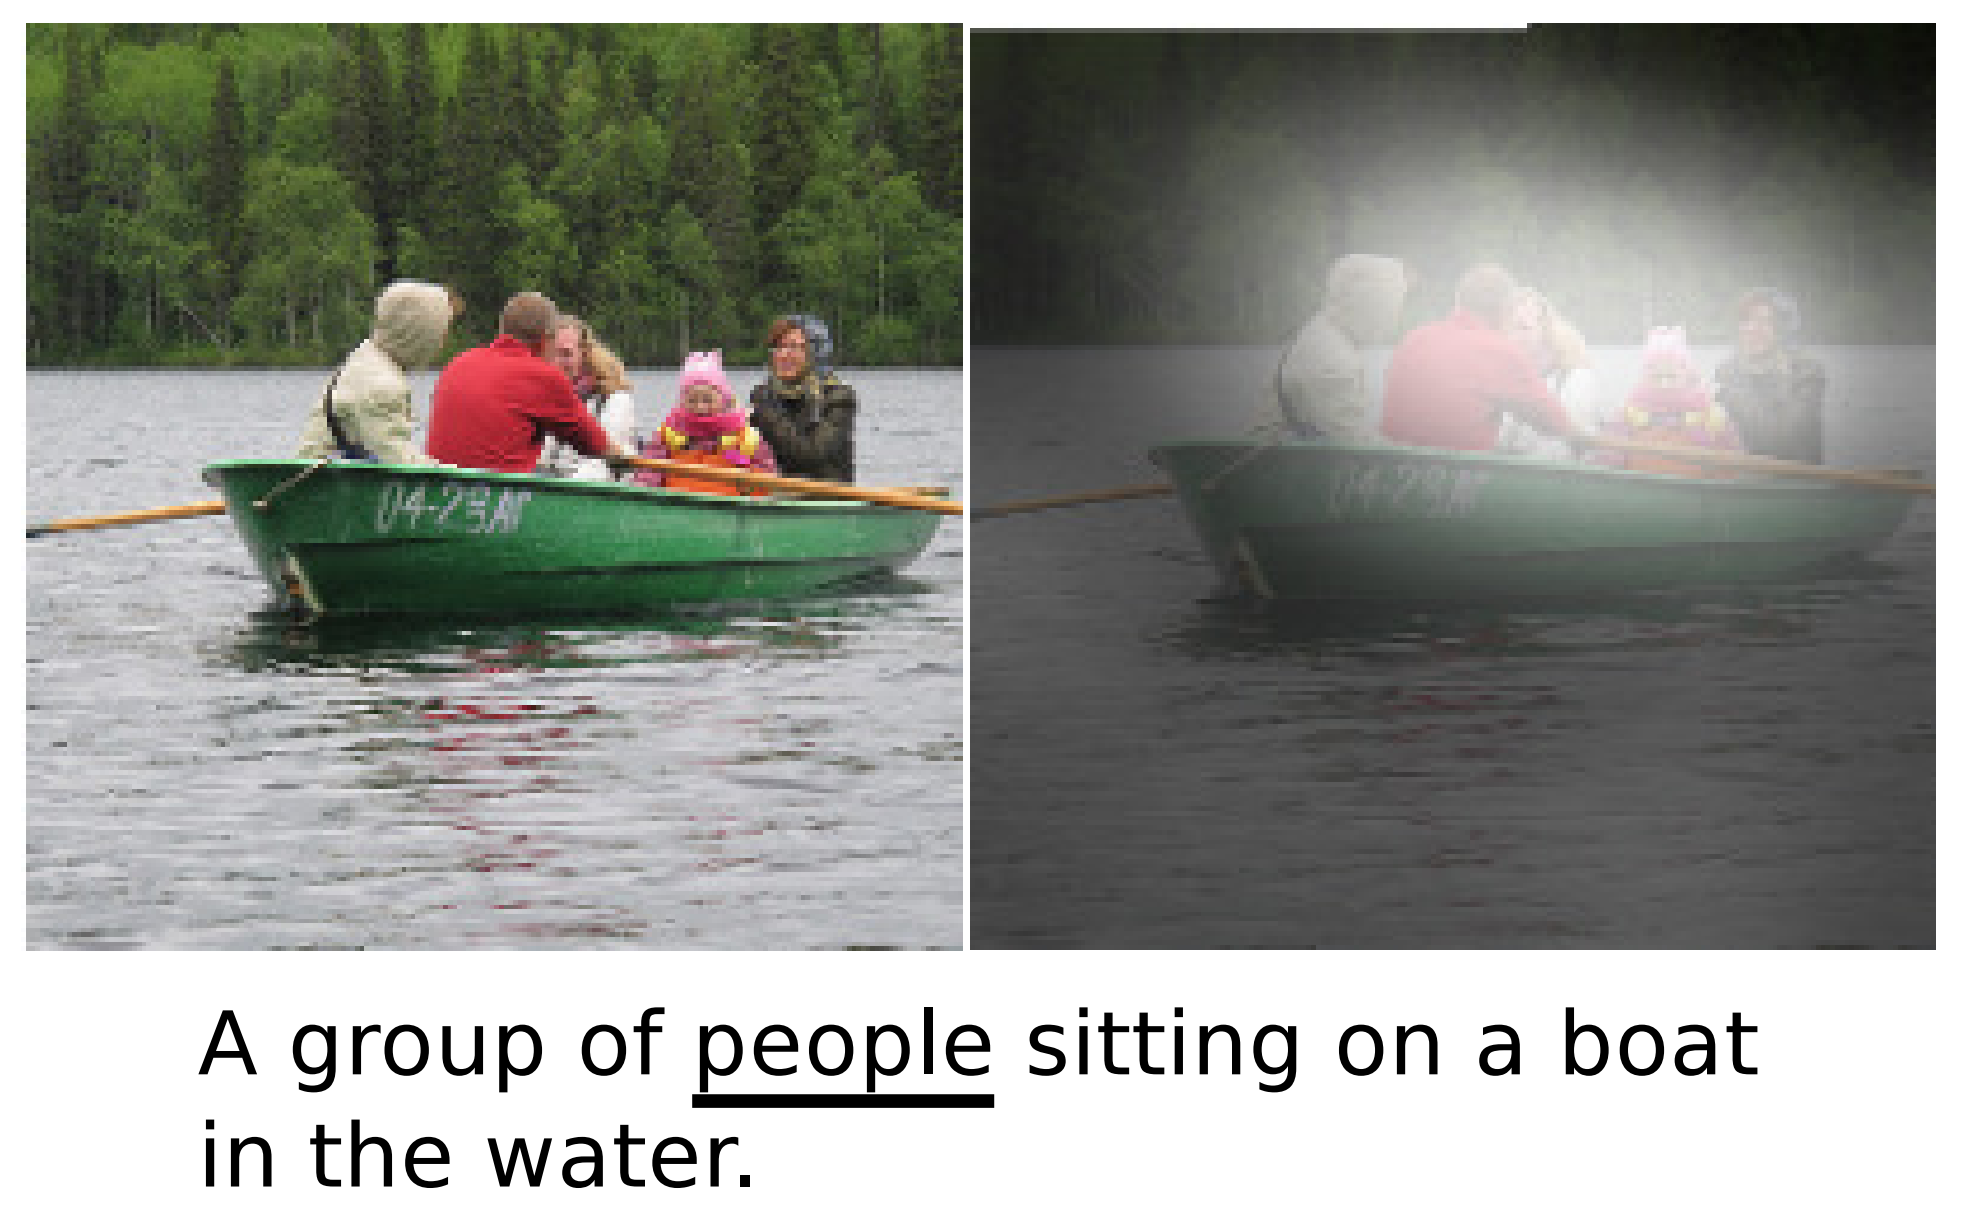
\includegraphics[width=5 cm, height=3.75cm]{caption.png}
	\caption{注意力权重可视化的一些例子.}
\end{figure*}
\section{注意力模型的应用}
注意力模型因其直观、多功能性和可解释性而成为研究的热点。注意力模型的变体已经被用来处理不同应用领域的独特特征,例如:文本总结、阅读理解、语言建模、句法分析等。我们讨论注意力模型在如下三个方面的应用:(1)自然语言生成(NLG); (2)分类;(3)推荐系统。


自然语言生成任务是将自然语言作为模型的输出。许多自然语言生成任务例如机器翻译,问答系统和多媒体数据描述已经受益于注意力机制的加入。机器翻译使用算法将文本或语音从一种语言翻译成另一种语言。机器翻译中的一个关键问题是如何用神经网络技术对注意力进行建模可以使不同语言的句子更好地对齐。相关研究表明,在翻译较长的句子时,注意力模型的优势也变得更加明显。通过将注意力机制引入问答系统,可以帮助模型通过注意更为重要的部分来理解问题,同时存储的大量信息也能够帮助问答系统找到合适的答案。此外通过协注意力模型对问答任务中的多模态数据进行建模也能够给提升系统的性能。


多媒体数据描述的任务场景是为多媒体输入序列生成一段自然语言形式的描述,其中的多媒体输入序列可以是语音、图像和视频。与问答系统类似,这里的注意力在语音或图像输入的相关部分寻找相关的声学信号,预测标题中的下一个单词。此外还可以利用多媒体数据比如视频数据的时空结构结合多层注意力机制来完成为视频取标题的任务。其中较低的层次用来捕捉视频帧中的特定区域,较高层次则用来抽取众多视频帧中的一个小子集。


文本分类任务和情感分析任务往往是基于一种自注意力模型从输入序列中找到与当前任务最为密切的元素来帮助对文本进行分类或者情感分析。


注意力模型也被广泛用于推荐系统的用户分析,即,为用户互动的项目分配注意力权重,以更有效地获取长期和短期兴趣。很明显并不是用户与项目的所有互动都与其对该项目的偏好有关并且用户的兴趣也会随着时间不断变化。多篇论文使用自注意机制寻找用户历史上最相关的条目,通过协同过滤框架改进条目检索;或在编码器-解码器架构内进行顺序推荐。


最近注意力被以新颖的方式使用,这为研究开辟了新的途径。一些有趣的方向包括如何更平滑地整合外部知识库、如何将预训练嵌入,如何进行多任务学习和无监督的表示学习、稀疏性学习和原型学习(比方说样本选择)。
\section{结论}
在本文,我们讨论了文献中描述注意力的不同方法,并试图通过讨论注意力的分类、使用注意力的关键神经网络架构以及已经看到显著影响的应用领域,来概述各种技术。我们讨论了在神经网络中引入注意力机制是如何使性能得到显著提高的。并且通过可视化注意力模块提高了模型的可解释性,从而对神经网络的内部工作有了更深入的了解,并介绍了一些方法如何通过消除输入的顺序处理提高了计算效率。


关于本文更为完整的版本请查看参考文献及参考文献中对各项工作的具体引用。
\end{document}